% ansatz1.tex
\section{ein erster Ansatz}
\begin{frame}
	\frametitle{Ansatz 1}
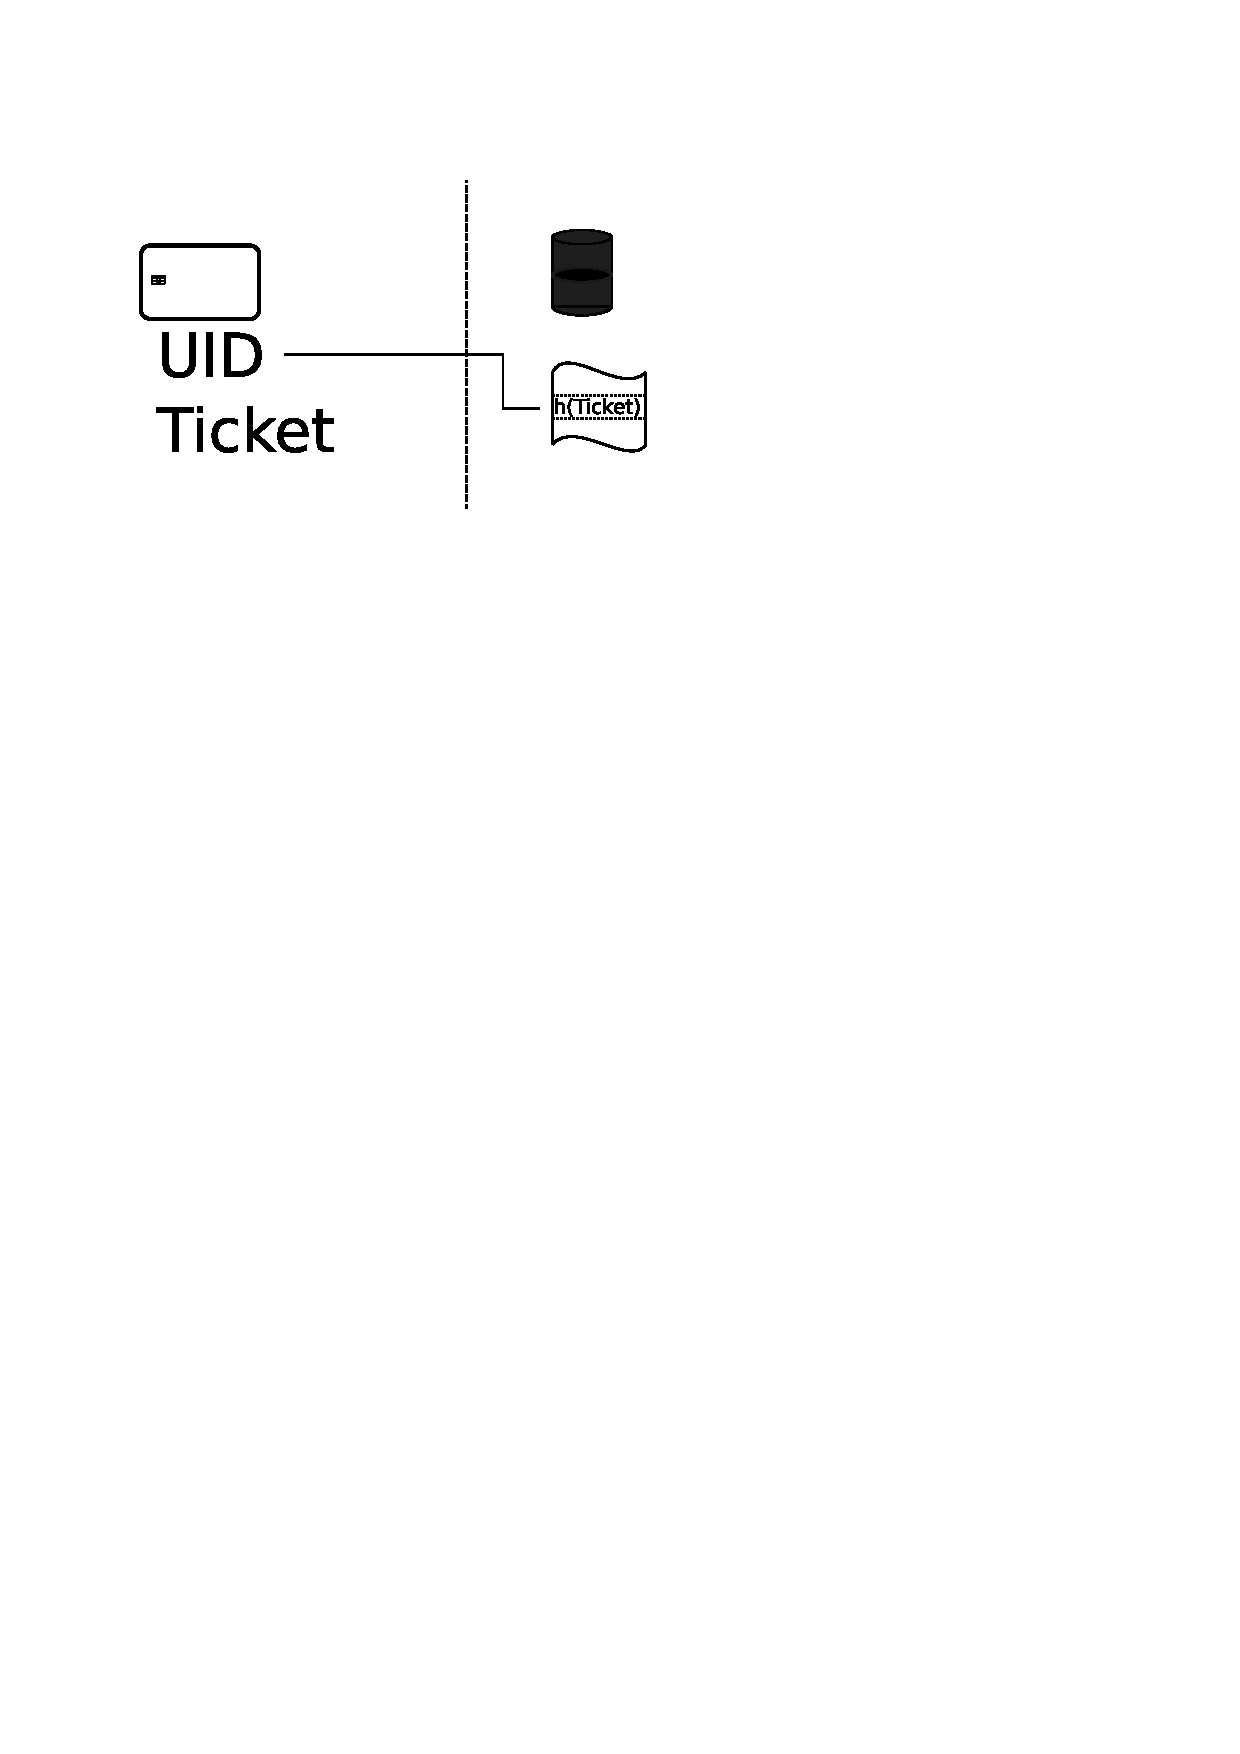
\includegraphics[scale=0.75]{ansatz1.pdf}
\end{frame}

\begin{frame}
	\frametitle{Ansatz 1 -- Ablauf}
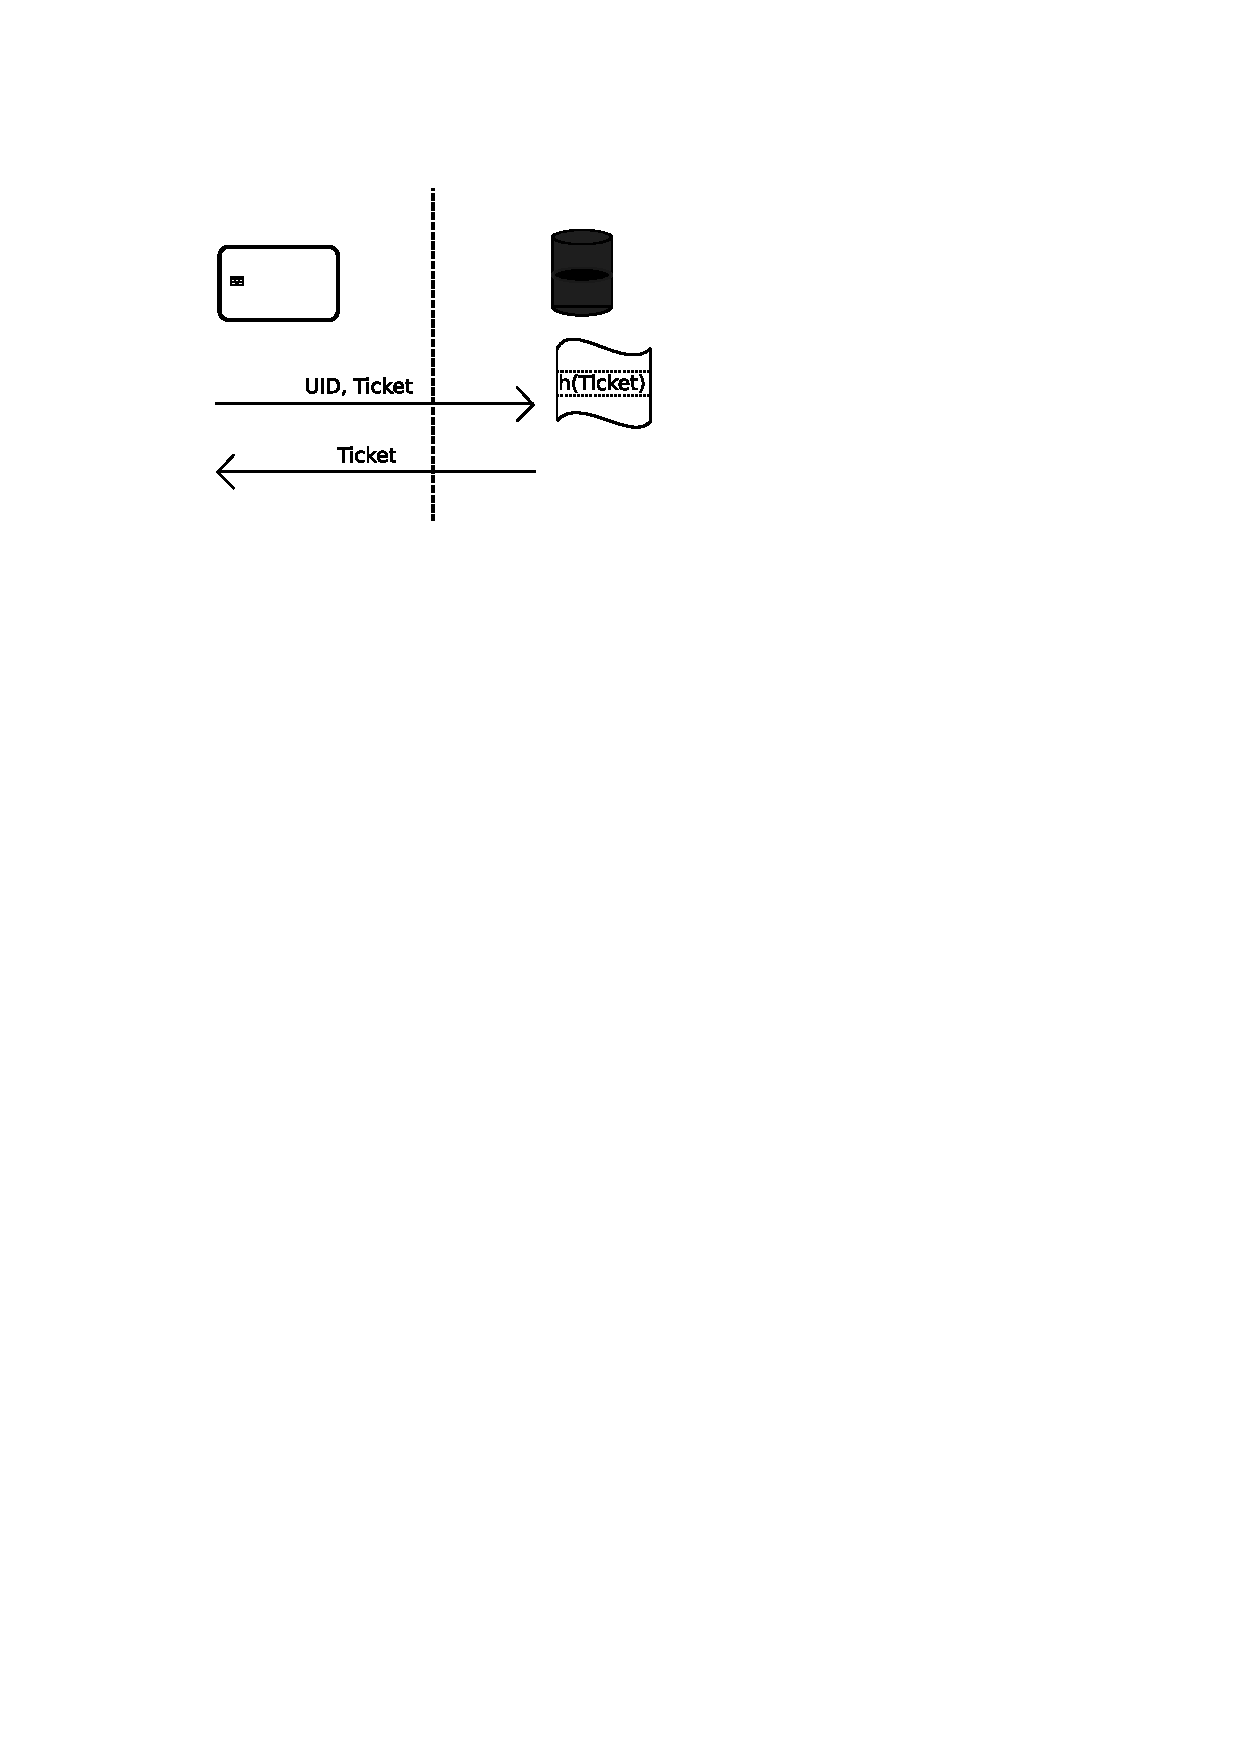
\includegraphics[scale=0.75]{ansatz1ablauf.pdf}
\end{frame}

\begin{frame}
	\frametitle{Ticket-DB Struktur}
%	uint8_t     flags;
%	uint8_t	    nickname[7];
%	ticketmac_t ticketmac;
Struktur eines Eintrags in der Ticket-DB:
\begin{tabular}{|c|c|}
\hline flags     & Flags (siehe unten) \\ 
\hline nickname  & Nickname (wenn Speicherung gewünscht) \\ 
\hline ticketmac & MAC vom Ticket \\ 
\hline 
\end{tabular} 

%	unsigned exist:1;				/* this user exists */
%	unsigned admin:1;				/* this user is admin */
%	unsigned locked:1;				/* this account is locked */
%	unsigned notify_lostadmin:1;	/* this user must be notifyed about lost admin privileges */
%	unsigned anonymous:1;			/* this user is anonymous */
%	unsigned reserved:3;
\vspace{1cm}
Struktur der Flags:
\begin{tabular}{|c|c|}
\hline exist     & Benutzer existiert \\ 
\hline admin     & Benutzer hat Admin Status \\ 
\hline locked    & Benutzer ist gesperrt \\ 
\hline notify\_lostadmin & Benutzer hat Admin Status verloren\\
\hline anonymous & Benutzer hat keinen Namen hinterlegt \\
\hline 
\end{tabular} 
\end{frame}

